\documentclass[a4paper, 12pt]{extarticle}

% Includes 
\usepackage[utf8]{inputenc} % UTF-8 encode 
\usepackage[english, russian]{babel}
\usepackage{geometry} % adjust page layout 
\usepackage{graphicx} 
\usepackage{hyperref} 
\usepackage{amsmath} % math formulas 
\usepackage{setspace} % for set line spacing 
\usepackage{indentfirst} % indent on a first line after the paragraph 
% \usepackage{pgfplots} % for plots 
\usepackage{listings} % for code listings 
\usepackage{xcolor} % colors (used for listings)
\usepackage{sourcecodepro} % for another monospaced font 
\usepackage{cmap} % for correct search in pdf


% debug
% \usepackage{showframe} % frame borders for demonstration 


%%% Custom commands
% commands for unnumbered sections
\newcommand{\usection}[1]{\section*{#1} \addcontentsline{toc}{section}{\protect\numberline{}#1}}
\newcommand{\usubsection}[1]{\subsection*{#1} \addcontentsline{toc}{subsection}{\protect\numberline{}#1}}
\newcommand{\usubsubsection}[1]{\subsubsection*{#1} \addcontentsline{toc}{subsubsection}{\protect\numberline{}#1}}


% Redefinition of section and subsection numbering style
\def\thesection{\arabic{section}.}
\def\thesubsection{\arabic{section}.\arabic{subsection}.}
\def\thesubsubsection{\arabic{section}.\arabic{subsection}.\arabic{subsubsection}.}



% Settings for links 
\hypersetup{
    colorlinks,
    citecolor=black,
    filecolor=black,
    linkcolor=black,
    urlcolor=black
}


% Layout
\geometry{
	left=17mm,
	top=17mm,
	right=17mm,
	bottom=20mm,
	marginparsep=0mm,
	marginparwidth=0mm,
	headheight=8mm,
	headsep=5mm, 
}

\linespread{1.5} % line spacing
\setlength{\parskip}{\baselineskip}  % Add space between paragraphs


% overfull hbox settings
\tolerance 10000 % default 200, max 10000
\hbadness 10000 % default 1000, max 10000
\emergencystretch 0pt  % default 0pt, how much the lines can stretch for the sake of good line breaks
\hfuzz 0.4pt % ignore overfull box less than 
\widowpenalty=10000 % no lines at the start of the page
\vfuzz \hfuzz % don't care about underfull vbox if overfull is acceptable
\raggedbottom % if the page is not filled, align the content to the bottom


% Redefinition of table of contents command to get centered heading
\makeatletter
\renewcommand\tableofcontents{ 
  \begin{singlespace}
    \null\hfill\textbf{\Large\contentsname}\hfill\null\par
    \@mkboth{\MakeUppercase\contentsname}{\MakeUppercase\contentsname}%
    \@starttoc{toc}
  \end{singlespace}
}
\makeatother


% Listings settings
\definecolor{codegreen}{rgb}{0, 0.6, 0}
\definecolor{codegray}{rgb}{0.5, 0.5, 0.5}
\definecolor{codepurple}{rgb}{0.58, 0, 0.82}
\definecolor{backcolour_gray}{rgb}{0.98, 0.98, 0.98}

\lstdefinestyle{python_white}{
  language=Python,
  backgroundcolor=\color{backcolour_gray},   
  commentstyle=\color{codegreen},
  keywordstyle=\color{blue},
  numberstyle=\tiny\color{codegray},
  stringstyle=\color{codepurple},
  basicstyle=\ttfamily\small\singlespacing,
  breakatwhitespace=true,         
  breaklines=true,                 
  captionpos=b, % t/b                  
  keepspaces=true,                 
  numbers=none, % none/left/rigth                    
  numbersep=5pt,                  
  showspaces=false,                
  showstringspaces=false,
  showtabs=false,                  
  tabsize=2,
  frame=single, % none/leftline/topline/bottomline/lines/single/shadowbox
  rulecolor=\color{gray}, % frame color 
}


\lstset{style=python_white}


% For title page
\def\name{Отчет по лабораторной работе №3} 
\def\subname{Фультрация Фурри через Фурье}
\def\madeby{Проворов Николай Дмитриевич, R3238}
\def\teacher{Перегудин А. А.}

\begin{document}

% Title page 
\begin{titlepage}

\thispagestyle{empty}

\title{


\includegraphics[width=4cm]{media/ITMO_logo.png} 

\vspace{1em}
НИУ ИТМО 
\vspace{4em}

\begin{center}
\large\textsc{\textbf{\name}}

\vspace{1em}
``\subname'' 

\end{center}

\vspace{7em}

\begin{flushright}
\normalsize{ 
Выполнил: \\ \textbf{\madeby} 

Преподаватель: \\ \textbf{\teacher} 
}
\end{flushright}	

\vspace{30pt}

\begin{center}
\small{Санкт-Петербург, \the\year}
\end{center}
}


\author{}
\date{}
\maketitle
\thispagestyle{empty}
\end{titlepage} % Title page

\tableofcontents % Table of contents
\pagebreak

\section{Фильтрация изображений с периодичностью}

Айоу, АКа, вот вам ... картинка с гугл диска, которая мне очень приглянулась.

\begin{figure}[ht!]
    \centering
    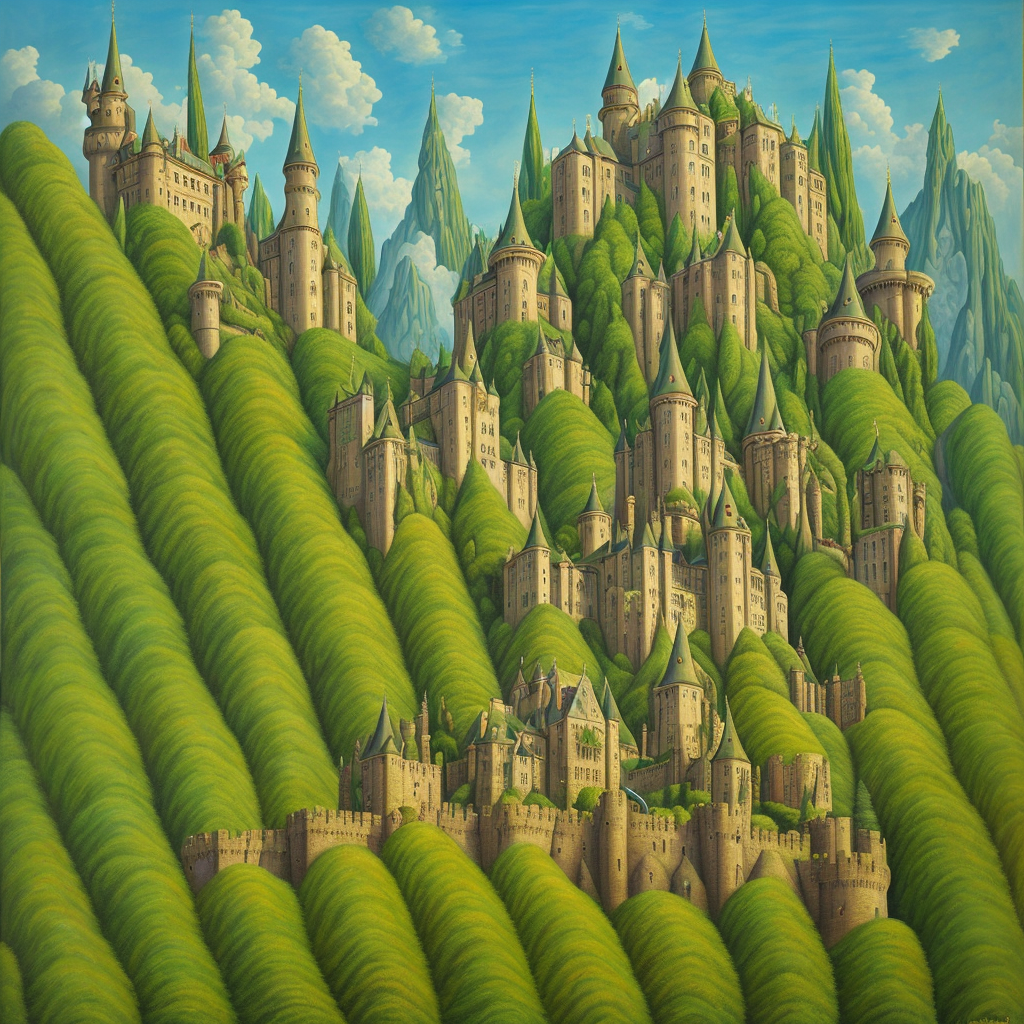
\includegraphics[width=1\textwidth]{/Users/nikolajprovorov/Yandex.Disk-368690@edu.itmo.ru.localized/Lab6_Furry_series/7.png}
    \caption{Картинка с гугл диска, которая мне очень приглянулась.}
    \label{fig:Source_img_1}
\end{figure}

Дальше по инструкции, работаем как сказано, но переписываем код под Python.

А вот и результат, мы получили фурье-образ изображения.

\begin{figure}[ht!]
    \centering
    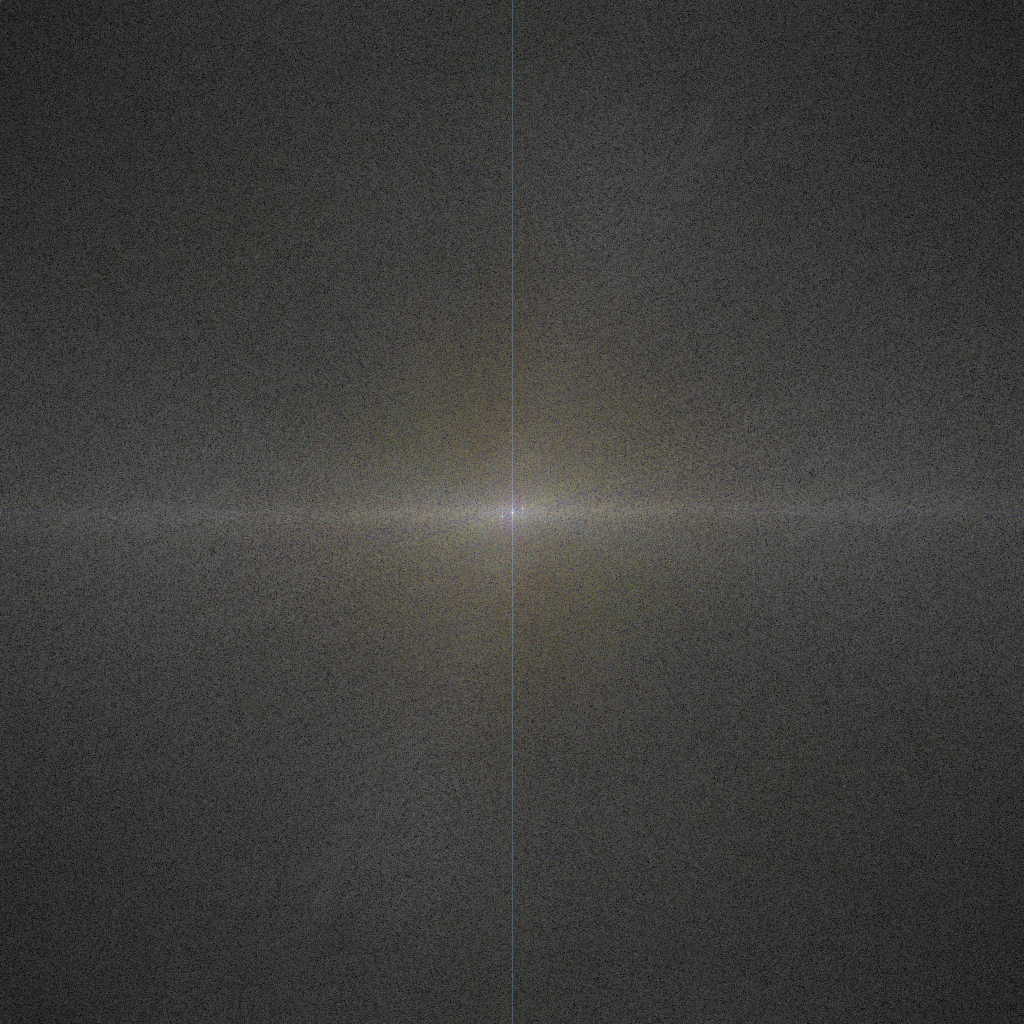
\includegraphics[width=1\textwidth]{/Users/nikolajprovorov/Yandex.Disk-368690@edu.itmo.ru.localized/Lab6_Furry_series/abs_fourier_log.png}
    \caption{Фурье-образ изображения.}
\end{figure}

\clearpage

На изображении присутсвует периодичность, которую мы можем убрать, если убрать пики. А вот и они:

\begin{figure}[ht!]
    \centering
    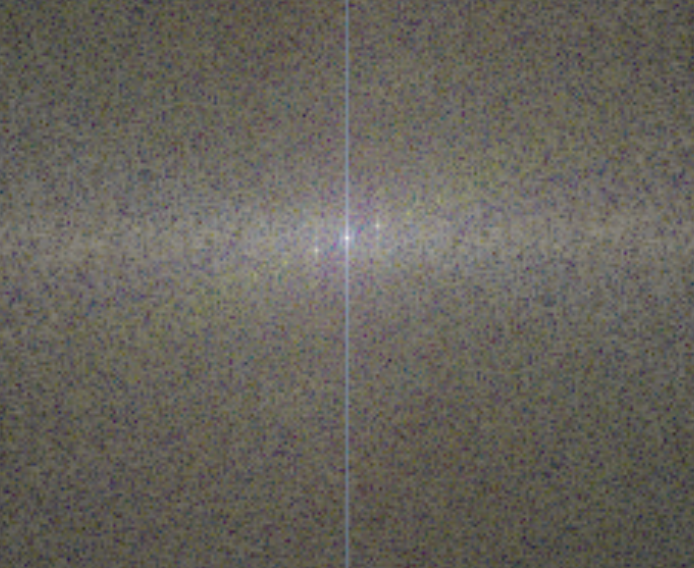
\includegraphics[width=1\textwidth]{/Users/nikolajprovorov/Yandex.Disk-368690@edu.itmo.ru.localized/Lab6_Furry_series/image.png}
    \caption{Пики.}
\end{figure}

Убрали в фотошопе, а вот и результат:

\clearpage

\begin{figure}[ht!]
    \centering
    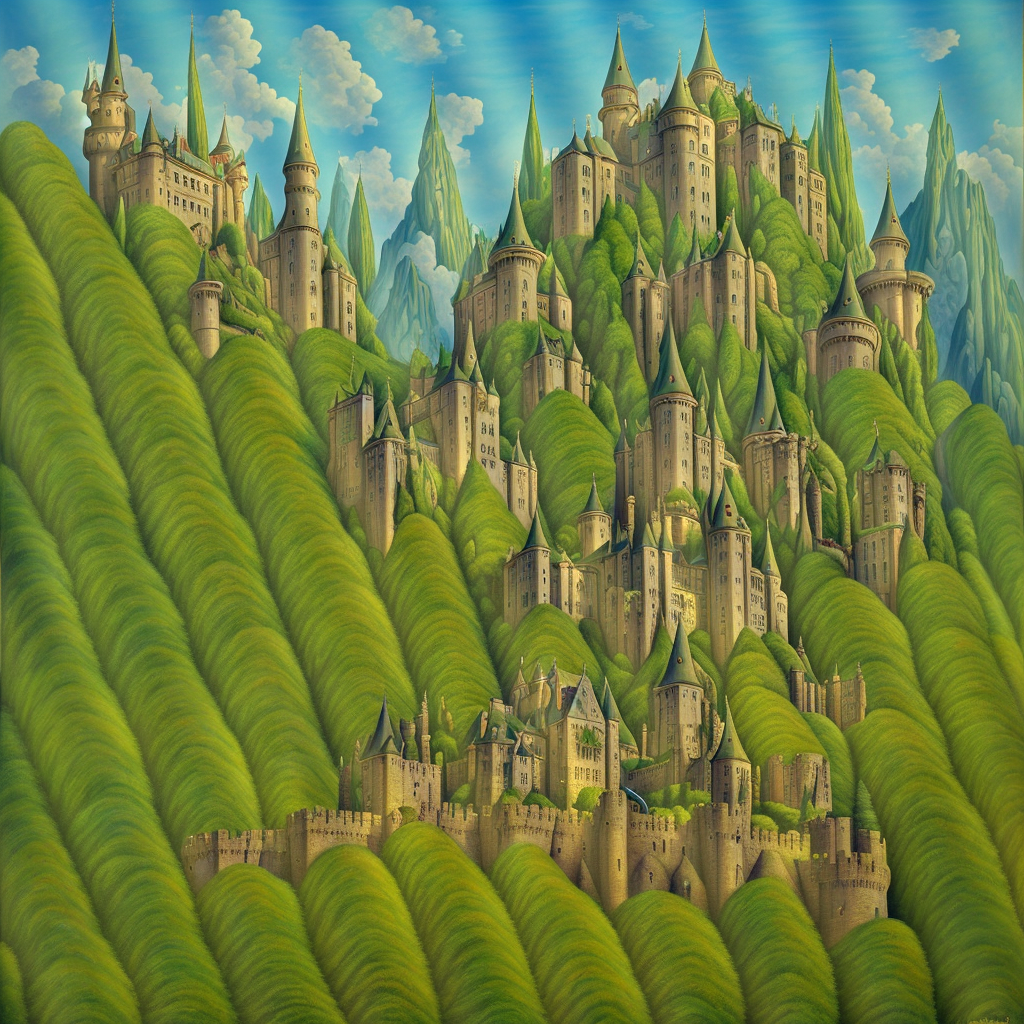
\includegraphics[width=1\textwidth]{/Users/nikolajprovorov/Yandex.Disk-368690@edu.itmo.ru.localized/Lab6_Furry_series/restored.png}
    \caption{Результат.}
\end{figure}

Стало лучше, и мне это нравится. Чуть изменилось само изображение, возможно мы затронули то, что не надо было, но уже ладно. Двигаемся дальше.



\clearpage

\section{Размытие изображения}

Для начала мы преобразуем изображение в черно-белое.

\begin{figure}[ht!]
    \centering
    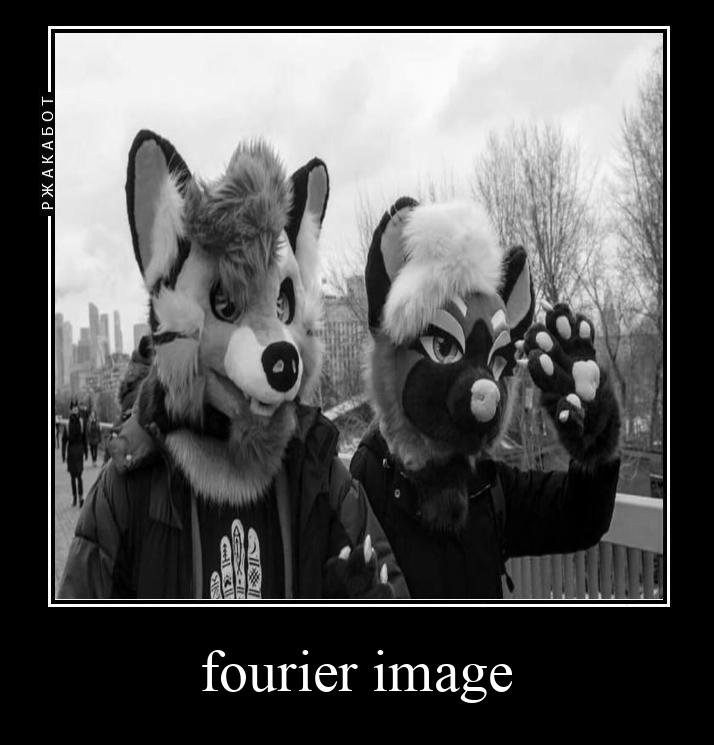
\includegraphics[width=0.5\textwidth]{/Users/nikolajprovorov/Yandex.Disk-368690@edu.itmo.ru.localized/Lab6_Furry_series/bw.png}
    \caption{Черно-белое изображение}
\end{figure}

Для начала выберу 3 нечетных значения $n = 3, 5, 7$

\subsection{Блочное размытие.}

Создадим 3 матрицы ядра блочного размытия. Для этого используем команду 

\begin{equation}
    ones(n)/(n^2)
\end{equation}

\clearpage

Посмотрим на результаты применения ядер к изображению.

\begin{figure}[ht!]
    \centering
    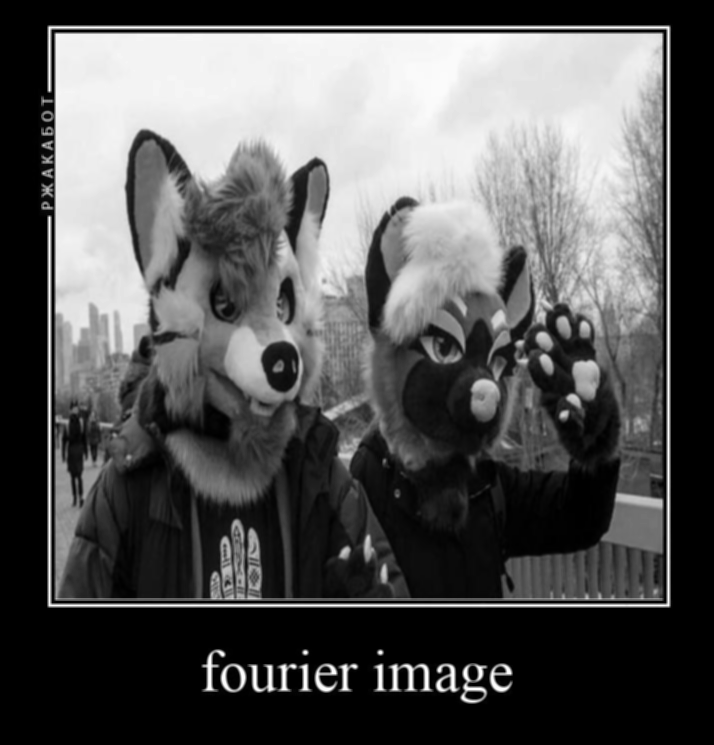
\includegraphics[width=0.5\textwidth]{/Users/nikolajprovorov/Yandex.Disk-368690@edu.itmo.ru.localized/Lab6_Furry_series/block_3.png}
    \caption{Блочное размытие с $n = 3$}
\end{figure}

\begin{figure}[ht!]
    \centering
    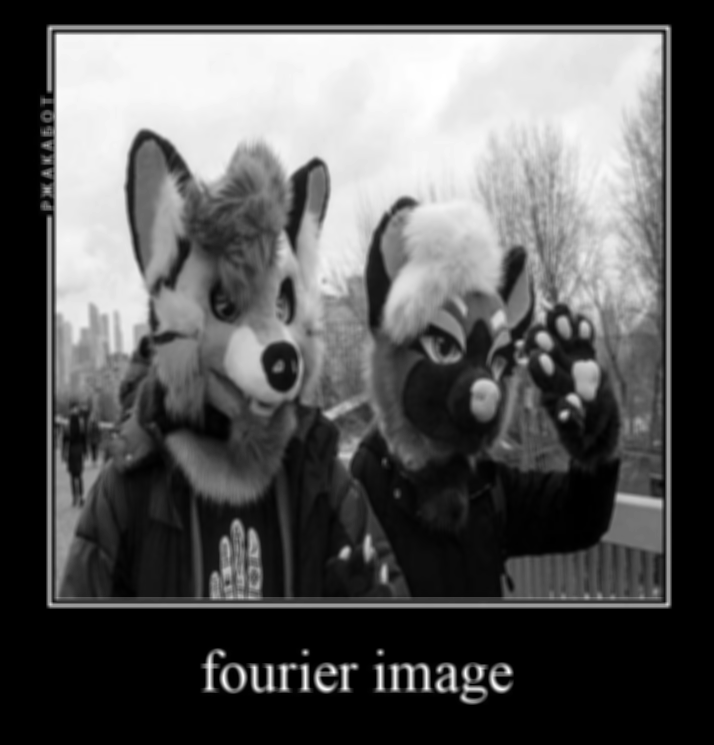
\includegraphics[width=0.5\textwidth]{/Users/nikolajprovorov/Yandex.Disk-368690@edu.itmo.ru.localized/Lab6_Furry_series/block_5.png}
    \caption{Блочное размытие с $n = 5$}
\end{figure}

\clearpage

\begin{figure}[ht!]
    \centering
    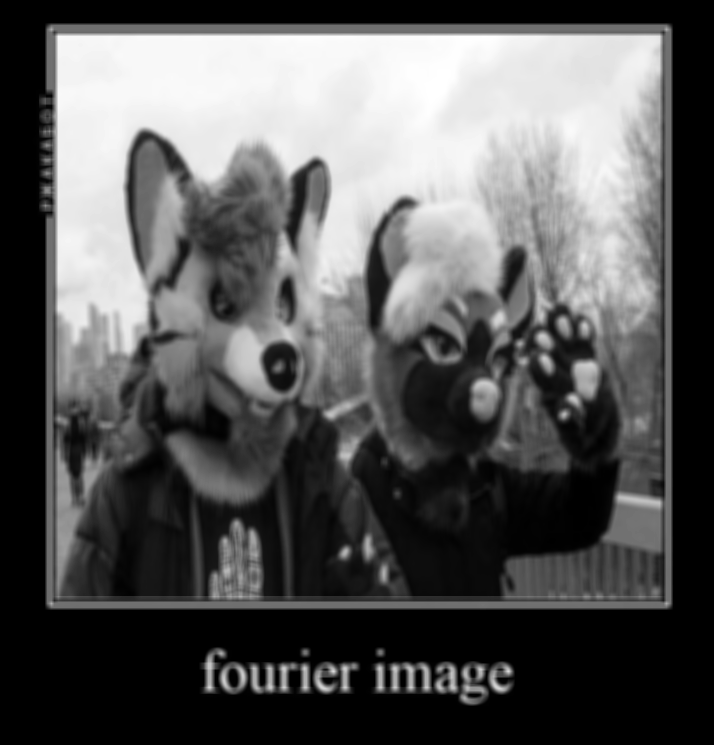
\includegraphics[width=0.5\textwidth]{/Users/nikolajprovorov/Yandex.Disk-368690@edu.itmo.ru.localized/Lab6_Furry_series/block_7.png}
    \caption{Блочное размытие с $n = 7$}
\end{figure}

\subsection{Размытие Гаусса.}

Применим фильтр Гаусса к изображению.

\begin{figure}[ht!]
    \centering
    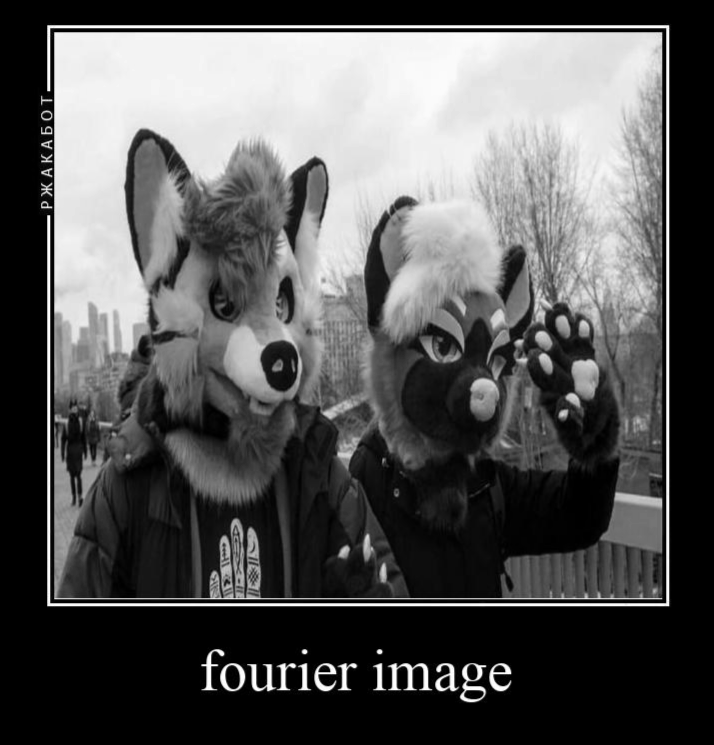
\includegraphics[width=0.5\textwidth]{/Users/nikolajprovorov/Yandex.Disk-368690@edu.itmo.ru.localized/Lab6_Furry_series/gaussian_3.png}
    \caption{размытие Гаусса с $n = 3$}
\end{figure}

\clearpage

\begin{figure}[ht!]
    \centering
    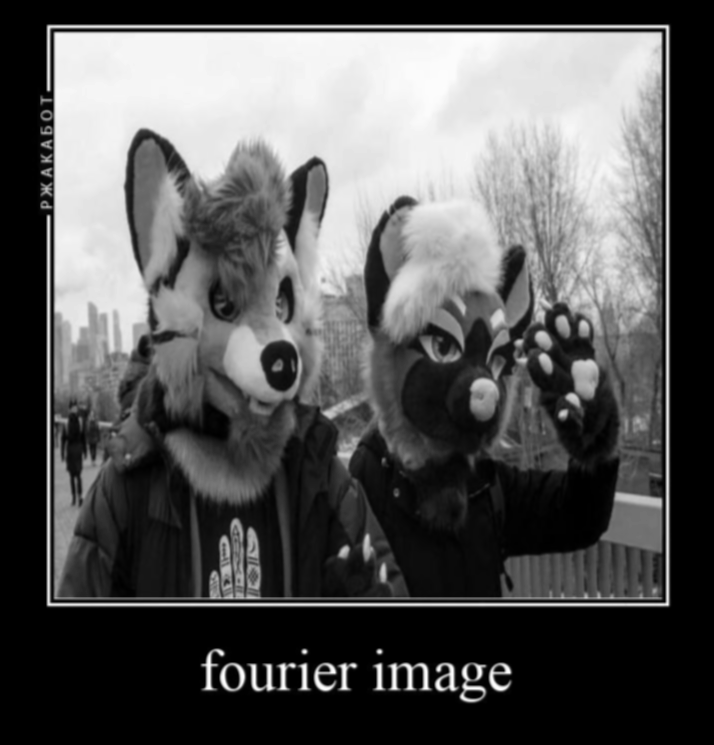
\includegraphics[width=0.5\textwidth]{/Users/nikolajprovorov/Yandex.Disk-368690@edu.itmo.ru.localized/Lab6_Furry_series/gaussian_5.png}
    \caption{размытие Гаусса с $n = 5$}
\end{figure}

\begin{figure}[ht!]
    \centering
    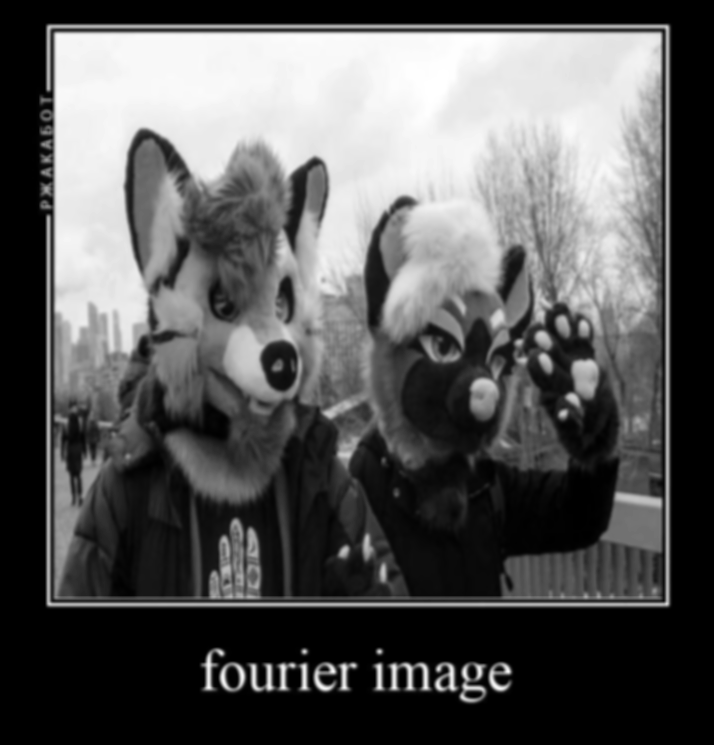
\includegraphics[width=0.5\textwidth]{/Users/nikolajprovorov/Yandex.Disk-368690@edu.itmo.ru.localized/Lab6_Furry_series/gaussian_7.png}
    \caption{размытие Гаусса с $n = 7$}
\end{figure}

\clearpage

Теперь посмотрм что там с фурье-котовасией.

\begin{figure}[ht!]
    \centering
    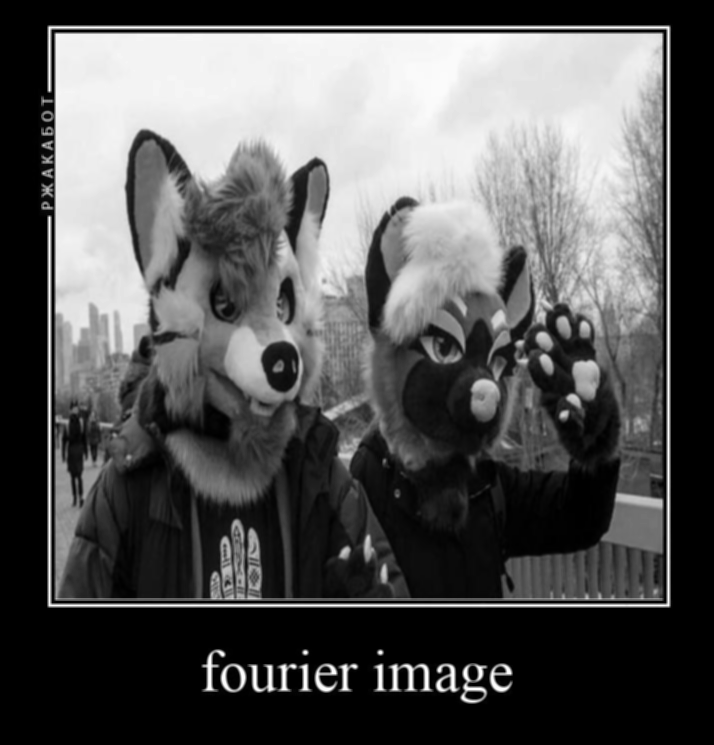
\includegraphics[width=0.5\textwidth]{/Users/nikolajprovorov/Yandex.Disk-368690@edu.itmo.ru.localized/Lab6_Furry_series/block_3.png}
    \caption{Блочное размытие с $n = 3$ (через фурье)}
\end{figure}

\begin{figure}[ht!]
    \centering
    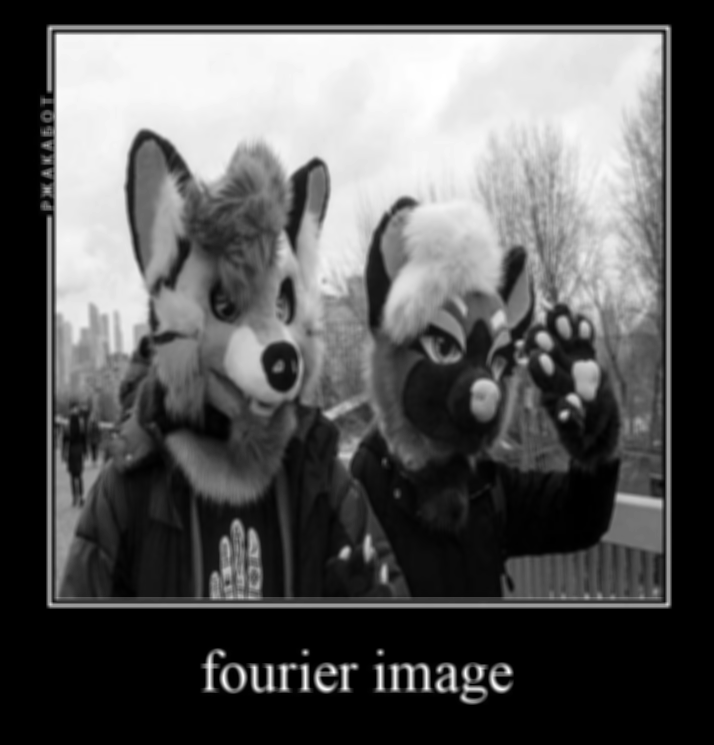
\includegraphics[width=0.5\textwidth]{/Users/nikolajprovorov/Yandex.Disk-368690@edu.itmo.ru.localized/Lab6_Furry_series/block_5.png}
    \caption{Блочное размытие с $n = 5$ (через фурье)}
\end{figure}

\clearpage

\begin{figure}[ht!]
    \centering
    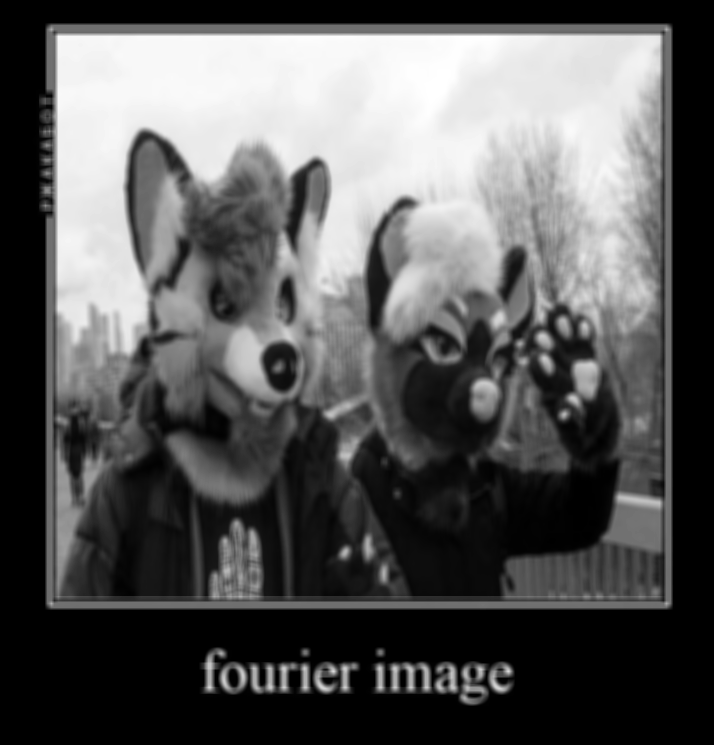
\includegraphics[width=0.5\textwidth]{/Users/nikolajprovorov/Yandex.Disk-368690@edu.itmo.ru.localized/Lab6_Furry_series/block_7.png}
    \caption{Блочное размытие с $n = 7$ (через фурье)}
\end{figure}

\begin{figure}[ht!]
    \centering
    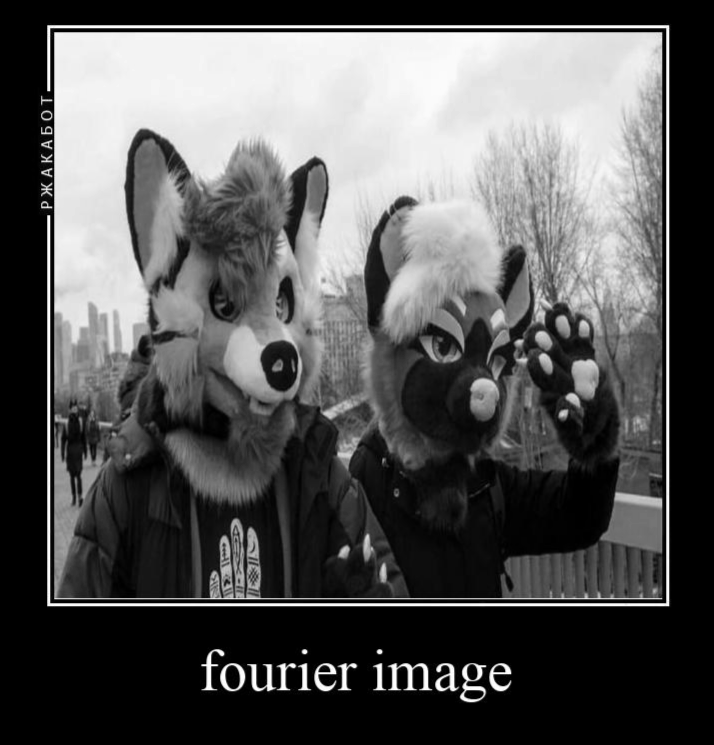
\includegraphics[width=0.5\textwidth]{/Users/nikolajprovorov/Yandex.Disk-368690@edu.itmo.ru.localized/Lab6_Furry_series/gaussian_3.png}
    \caption{размытие Гаусса с $n = 3$ (через фурье)}
\end{figure}

\clearpage

\begin{figure}[ht!]
    \centering
    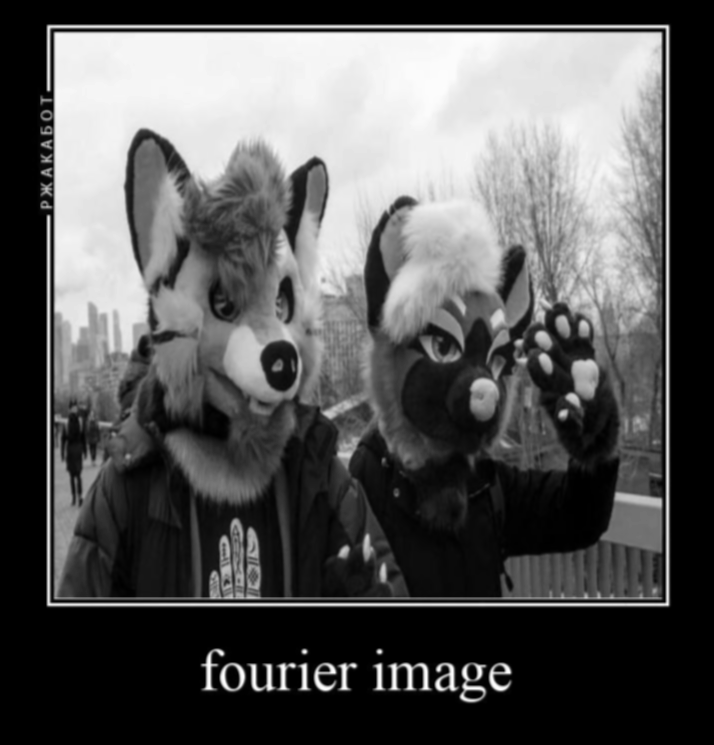
\includegraphics[width=0.5\textwidth]{/Users/nikolajprovorov/Yandex.Disk-368690@edu.itmo.ru.localized/Lab6_Furry_series/gaussian_5.png}
    \caption{размытие Гаусса с $n = 5$ (через фурье)}
\end{figure}

\begin{figure}[ht!]
    \centering
    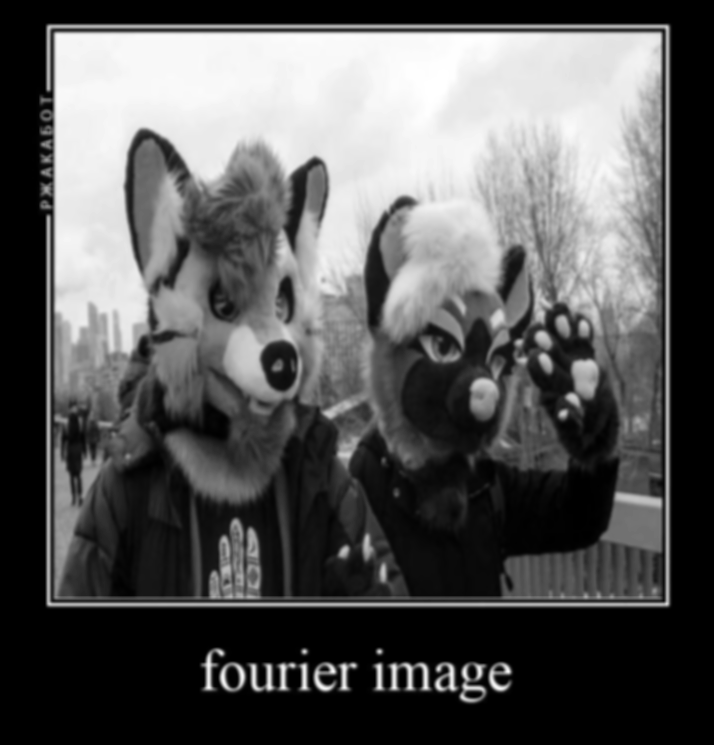
\includegraphics[width=0.5\textwidth]{/Users/nikolajprovorov/Yandex.Disk-368690@edu.itmo.ru.localized/Lab6_Furry_series/gaussian_7.png}
    \caption{размытие Гаусса с $n = 7$ (через фурье)}
\end{figure}

Результаты совпадают, прикольно. Все работает.

Если сравнивать блочное размытие с Гауссом, то можно заметить, что Гауссовское размытие более плавное, чем блочное. Также Гауссовское размытие не так сильно ухудшает качество изображения, как блочное.

\clearpage

\section{Увеличение резкости изображения}

Для начала мы преобразуем изображение в черно-белое.

\begin{figure}[ht!]
    \centering
    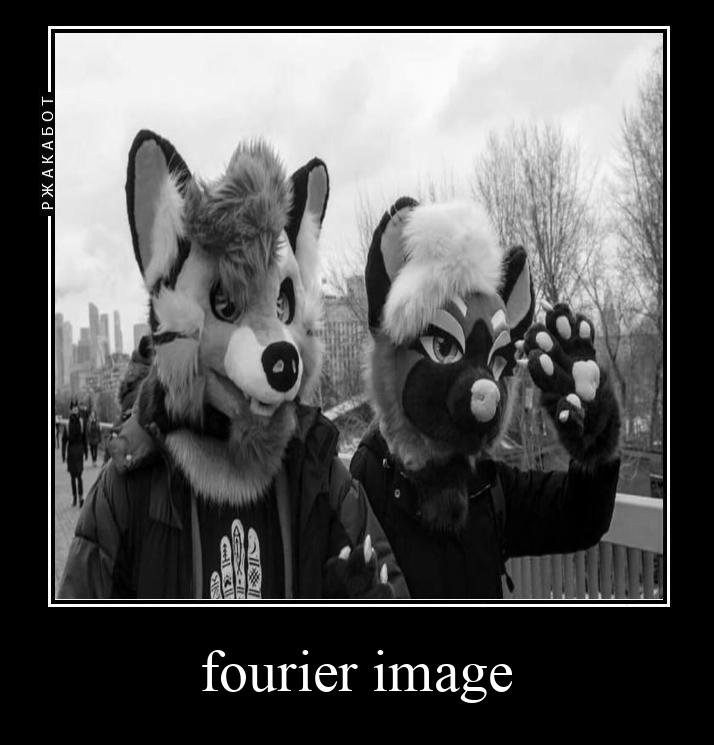
\includegraphics[width=0.5\textwidth]{/Users/nikolajprovorov/Yandex.Disk-368690@edu.itmo.ru.localized/Lab6_Furry_series/bw.png}
    \caption{Черно-белое изображение}
\end{figure}

Зададим матрицу ядра увеличния резкости:

\begin{equation}
    K = 
    \begin{bmatrix}
        0 & -1 & 0 \\
        -1 & 5 & -1 \\
        0 & -1 & 0
    \end{bmatrix}
\end{equation}

Посмотрим на результат применения:

\clearpage

\begin{figure}[ht!]
    \centering
    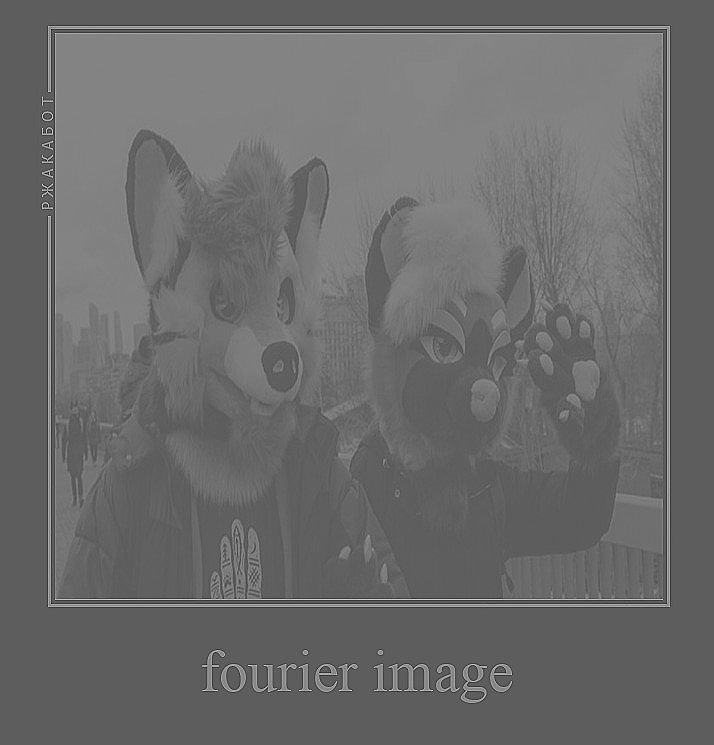
\includegraphics[width=0.5\textwidth]{/Users/nikolajprovorov/Yandex.Disk-368690@edu.itmo.ru.localized/Lab6_Furry_series/laplacian.png}
\end{figure}

Стало явно лучше, резкость увеличилась, но изображение потеряло в контрасте.

Давайте посмотрим теперь на результат всего вот того фурье:

\begin{figure}[ht!]
    \centering
    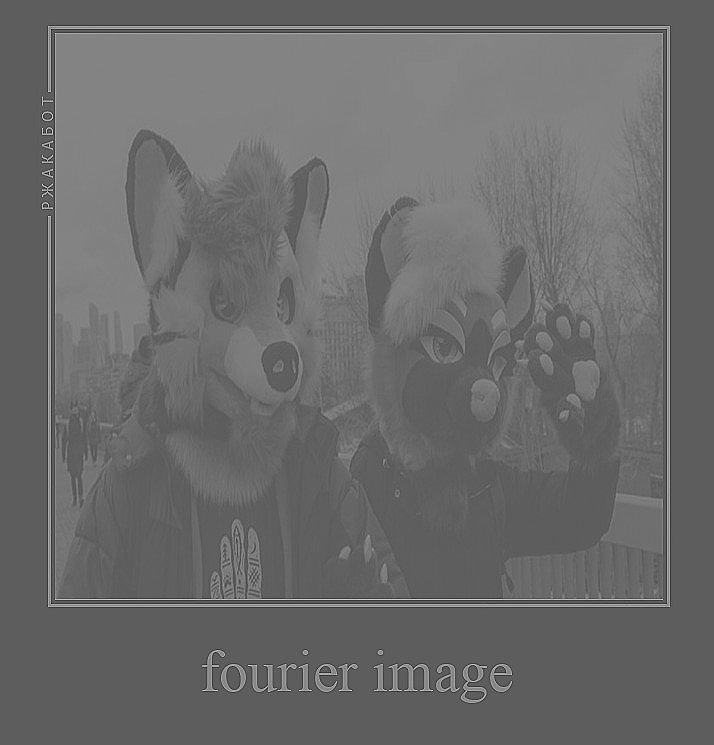
\includegraphics[width=0.5\textwidth]{/Users/nikolajprovorov/Yandex.Disk-368690@edu.itmo.ru.localized/Lab6_Furry_series/laplacian.png}
    \caption{Увеличение резкости изображения что-то там фурье}
\end{figure}

О, прикол, совпали. Теорема о свертке работает корректно.

\clearpage

\section{Выделение краев изображения}

Для начала мы преобразуем изображение в черно-белое.

\begin{figure}[ht!]
    \centering
    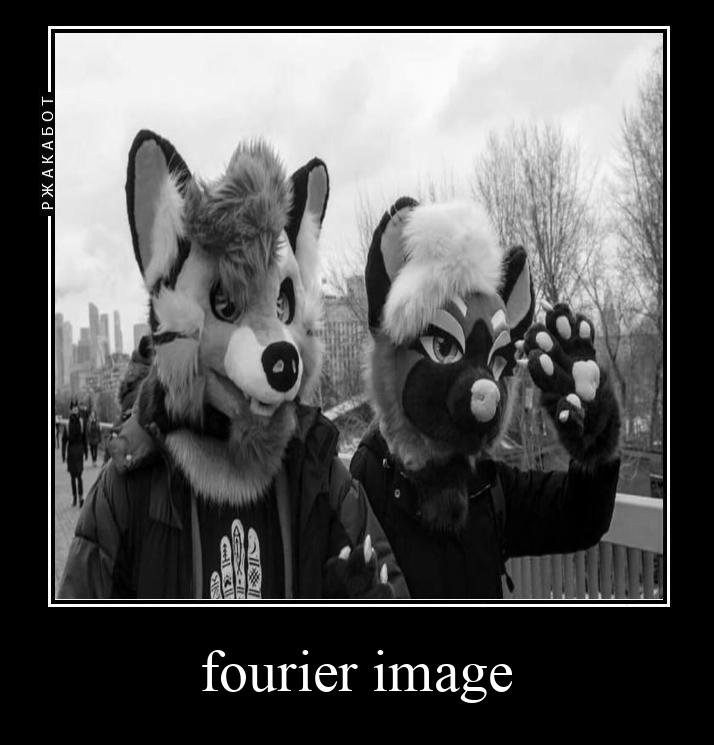
\includegraphics[width=0.5\textwidth]{/Users/nikolajprovorov/Yandex.Disk-368690@edu.itmo.ru.localized/Lab6_Furry_series/bw.png}
    \caption{Черно-белое изображение}
\end{figure}

Зададим матрицу ядра выделения краев:

\begin{equation}
    K = 
    \begin{bmatrix}
        -1 & -1 & -1 \\
        -1 & 8 & -1 \\
        -1 & -1 & -1
    \end{bmatrix}
\end{equation}

Найдем свертку исходного изображения с ядром и тд и тп, короче вот результат:

\clearpage

\begin{figure}[ht!]
    \centering
    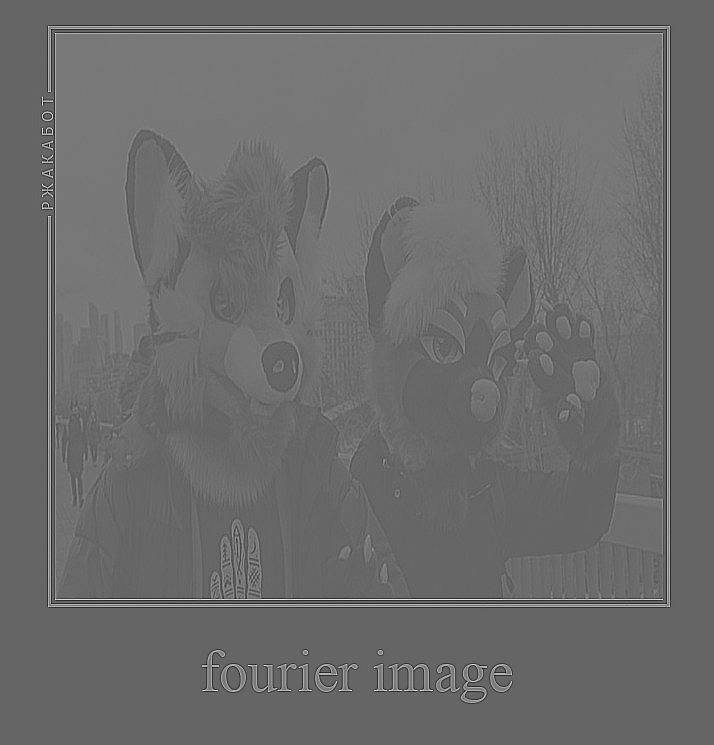
\includegraphics[width=0.5\textwidth]{/Users/nikolajprovorov/Yandex.Disk-368690@edu.itmo.ru.localized/Lab6_Furry_series/edge_x.png}
    \caption{Выделение краев изображения}
\end{figure}

Ну получилось очень даже неплохо, контрастность конечно пострадала, и сильно, но зато какие края!

Давайте посмотрим теперь на результат всего вот того фурье:

\begin{figure}[ht!]
    \centering
    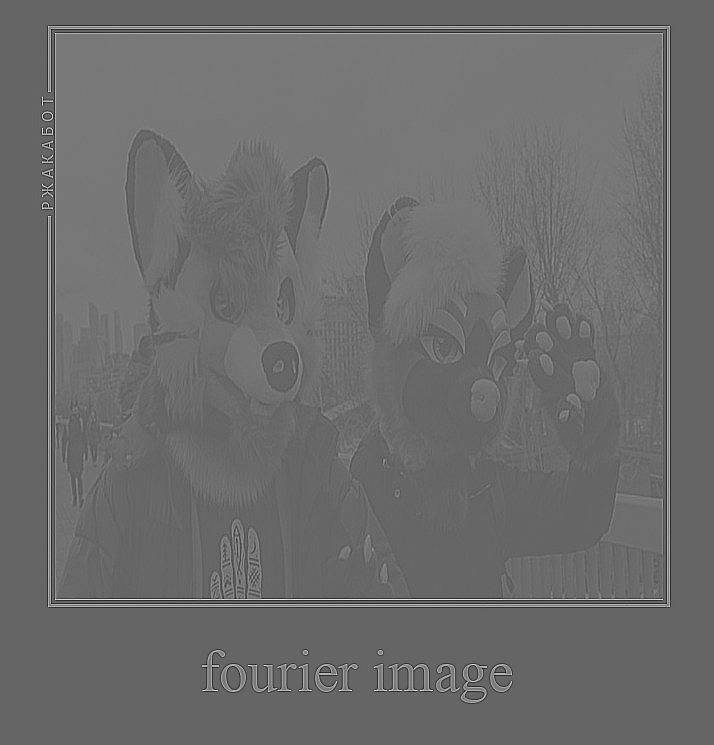
\includegraphics[width=0.5\textwidth]{/Users/nikolajprovorov/Yandex.Disk-368690@edu.itmo.ru.localized/Lab6_Furry_series/edge_x.png}
    \caption{Выделение краев изображения}
\end{figure}

О, прикол, совпали. Теорема о свертке работает корректно.

\clearpage

В целом, так как это последняя лабораторная по данному предмету, хочу сказать вам спасибо. 

\begin{figure}[ht!]
    \centering
    
\includegraphics[width=1\textwidth]{/Users/nikolajprovorov/Yandex.Disk-368690@edu.itmo.ru.localized/Lab6_Furry_series/Unknown.jpeg}
    \caption{Спасибо за внимание.}
\end{figure} % Content

\end{document}